\setcounter{page}{1}
\chapter{Introduction}\label{sec:introduction}

The Lightning Network is a peer-to-peer protocol designed to
provide a scalable solution to allow Bitcoin micro-transactions.
Bitcoin, a digital currency created in 2009, uses blockchain technology
to track and verify transactions. The blockchain is a secure and transparent
record of all transactions that have ever occurred on the network.

Bitcoin has long suffered from scalability limitations, which have been
addressed in various ways, including hard forks of the protocol.
The Lightning Network was proposed as an off-chain solution to Bitcoin's
scalability problems, enabling peers to exchange partially signed transactions
without violating Bitcoin rules.

However, despite the Lightning Network's potential, there is still a need
to make the Bitcoin protocol more scalable to compete with modern payment systems.
One approach to improving the Lightning protocol over time is through making changes
to the protocol itself, and the underlying protocol such as Bitcoin. However,
implementing these kinds of changes to a protocol such as the Lightning Network
can take time and evaluation of different ideas.

In addition, currently, the {\LN} lacks public data to involve researchers
where they can evaluate different kinds of protocol proposals and
potential impact on the network. We introduce in Chapter \ref{sec:problem_and_state_of_the_art}
two problems where having public data on real Lightning Network nodes can be valuable.

Therefore, this lack of data restricts access to research topics for
people not strictly involved in the Lightning Network protocol development.
To address this need, this thesis aims to develop a collection of tools for
running Lightning Network nodes with daily activity. The data collected by
Lightning Network users will be analyzed by one or more centralized
analysis systems.

To perform this analysis, it is essential to involve the Lightning Network
community, particularly those running real nodes with real Bitcoin involved,
to obtain a realistic vision of the sub-network. 
One of the goals of this thesis is to develop a collection of 
tools are designed to run on nodes with daily activity to 
collect real node data.

Another goal is to define and collect Lightning Network
metrics to understand daily node performance better. 

We propose an open-source framework
for defining and collecting these metrics to meet these goals. The framework
is implemented through a lnmetrics Request for Comments (RFC), where is it possible to define
in a formal way the metric data and to iterate on the data format with the help of a community.
The data is collected by using a public server with a public API, with the possibility to
self-host the server on hardware with at least Raspberry PI 2 capability.

In contrast, the analysis of the Bitcoin blockchain requires more than
500 GB of space just to store the blockchain, as Figure \ref{fig:blockchain_size} shows,
and the space required can increase by over 1 TB if the blockchain is analyzed.

\begin{figure}[h]
  \begin{center}
    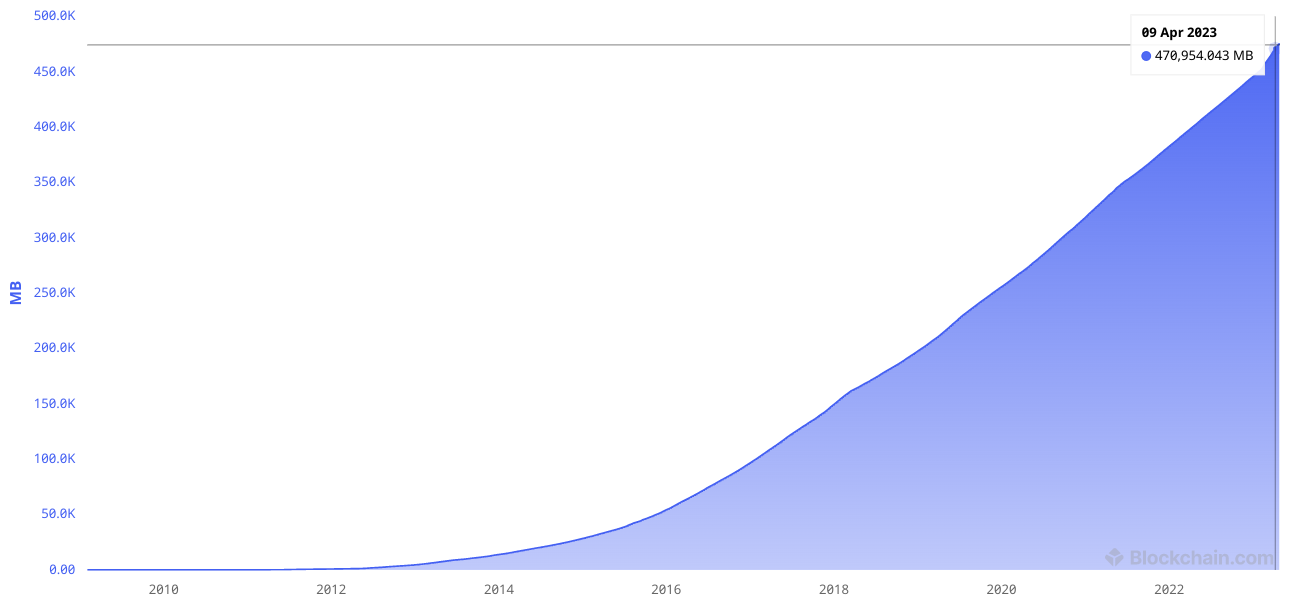
\includegraphics[width=0.6\columnwidth]{imgs/bitcoin-blockchain-size.png}
  \end{center}
  \caption{Bitcoin Blockchain size}
  \label{fig:blockchain_size}
\end{figure}

Our solution is heavily based on compression due to storing redundant JSON received
by the Lightning Network nodes. Due to the small space needed, we can run our solution on a
wide range of common hardware. We discuss the space requirements in Chapter \ref{chap:propsol}.
Therefore, the lower resource consumption and the possibility of receiving data from a
centralized server also allow for a lower level of expertise required to conduct small
research for the Lightning Network. This also enables bachelor students to conduct
experiments, not just with a theoretical scope, in the near future.

In addition, to incentivize node operators to provide and share their information, we allow our
tools to run in an offline mode with the possibility to calculate the proposed metrics on the
local machine without sharing information with the centralized analysis system. This incentive
is a core concept to allow for contributions from big users of the Lightning Network who are
seeking tools to increase their node's profit.

In the following chapters, we provide a comprehensive exploration of the Bitcoin protocol
(Chapter \ref{chap:bitcoin}), followed by an introduction to the Lightning Network
(Chapter \ref{sec:lightning_network}), which offers a potential solution to scaling issues
in Bitcoin. We then examine the specific problem we are addressing and review the current
state of the art (Chapter \ref{sec:problem_and_state_of_the_art}). Subsequently, we propose
a detailed solution (Chapter \ref{chap:propsol}), which utilizes specific technologies
(Chapter \ref{chap:tech}), and discuss possible future developments in our concluding chapter
(Chapter \ref{chap:conclusion}). Overall, our thesis presents a comprehensive analysis of the
Bitcoin protocol explores potential solutions to its scalability issues and offers a novel
solution that addresses a specific problem to allow more accessible data to researchers of the
field.

\section*{Our Contribution}

\begin{itemize}
  \item We introduce a general framework for \textbf{defining, collecting, and analyzing Lightning Network Metrics}.
        This framework drives data analyses on the Lightning Network and establishes a general process for proposing metrics
        to achieve consensus across different implementations.
  \item We contribute to \textbf{developing basic tools for Lightning Network research}. We develop the client that runs
        on a Lightning Network node \cite{lnmetrics-client}, implement a server \cite{lnmetrics-server} to aggregate and
        analyze metrics, and initiate the Request for Comment (RFC) initiative \cite{lnmetrics-rfc}.
  \item We contribute to the research community by \textbf{providing access to real-node Lightning Network data},
        which is typically rare to obtain due to the need for Lightning nodes with real Bitcoin involvement.
  \item We collaborate with the Lightning Network community \cite{lightning-network-ml-post-on-jamming} by \textbf{proposing
        lnmetrics as a framework to analyze the different metrics} proposed to mitigate the Channel Jamming Problem \cite{cryptoeprint:2022/1454}.
  \item We contribute to the core lightning ecosystem by \textbf{developing a new modular Go language API} \ref{sec:go-api}
        that improves performance when interacting with core lightning.
  \item We provide an \textbf{initial Lightning Network Metric called \emph{Local Reputation} \cite{lnmetrics_localreputation}
        to support Lightning Network users} in managing their Lightning Node.
  \item Finally, we provide an \textbf{initial analysis of data collected from a real Lightning Network Node}, making it available
        through a Jupyter Notebook \cite{lnmetrics-jupyter} and an interactive website at \url{https://lnmetrics.info}.
\end{itemize}
